\documentclass[12pt, fullpage,letterpaper]{article}

\usepackage[margin=1in]{geometry}
\usepackage{url}
\usepackage{amsmath}
\usepackage{amsfonts}
\usepackage{amssymb}
\usepackage{xspace}
\usepackage{graphicx}
\usepackage{bm}

%table position
\usepackage{float}
%multi columns
\usepackage[english]{babel}
\usepackage{multicol}
%caption without figure number
\usepackage{caption}
%drawing trees
\usepackage{tikz}
\usetikzlibrary{calc, shapes, backgrounds}
%merge cells
\usepackage{booktabs}
\usepackage{multirow}
%long table
\usepackage{longtable}
%code
\usepackage{listings}

\newcommand{\semester}{Spring 2018}
\newcommand{\assignmentId}{2}

\newcommand{\bx}{{\bf x}}
\newcommand{\by}{{\bf y}}
\newcommand{\bw}{{\bf w}}
\newcommand{\bu}{{\bf u}}

\title{CS 5350/6350: Machine Learining \semester}
\author{Homework \assignmentId\ Solutions\\\\Yulong Liang (u1143816)}

\begin{document}
\maketitle

\section{Expressiveness of Linear Classifiers}
\begin{enumerate}
\item~[60 points] 
\begin{enumerate}
\item $f(x_1, x_2, x_3) = x_1 \lor x_2 \lor x_3$
$$\bw=(1,1,1) \quad bias=-1 \quad x_1+x_2+x_3-1=0$$
\item $f(x_1, x_2, x_3) = x_1 \land \neg x_2 \land \neg x_3$
$$\bw=(1,-1,-1) \quad bias=-1 \quad x_1-x_2-x_3-1=0$$
\item $f(x_1, x_2, x_3) = \neg x_1 \lor \neg x_2 \lor \neg x_3$
$$\bw=(-1,-1,-1) \quad bias=2 \quad -x_1-x_2-x_3+2=0$$
\item $f(x_1, x_2, \ldots, x_n) = x_1 \lor x_2 \ldots \lor x_k$ (note that  $k <n$)
$$\bw=(\underbrace{1,1,\cdots,1}_\text{1 to k},\underbrace{0,0,\cdots,0}_\text{k+1 to n})\in \mathbb{R}^n \quad bias=-1$$
$$x_1+x_2+x_3+\cdots+x_k-1=0,\qquad i.e. \sum_{i=1}^kx_i-1=0$$
\item $f(x_1, x_2, x_3, x_4) = (x_1 \lor x_2) \land (x_3 \lor x_4)$\\
The above boolean function can be represented by, 
$$x_1+x_2\ge1\quad\mathbf{and}\quad x_3+x_4\ge1$$
This is a space defined by two different hyperplanes in $\mathbb{R}^4$,
$$x_1+x_2-1=0\quad and \quad x_3+x_4-1=0$$
Namely, it is the \textbf{intersection} of the positive sides of the \textbf{two hyperplanes}, which is not linear. So we CANNOT find such a linear classifier.
\item $f(x_1, x_2, x_3, x_4) = (x_1 \land x_2) \lor (x_3 \land x_4)$\\
The above boolean function can be represented by, 
$$x_1+x_2\ge2\quad\mathbf{or}\quad x_3+x_4\ge2$$
This is a space defined by two different hyperplanes in $\mathbb{R}^4$,
$$x_1+x_2-2=0\quad and \quad x_3+x_4-2=0$$
Namely, it is the \textbf{union} of the positive sides of the \textbf{two hyperplanes}, which is not linear. So we CANNOT find such a linear classifier.
\end{enumerate}
\item~[50 points]
\begin{enumerate}
\item $f(x_1, x_2, x_3) = x_1 \lor x_2 \lor x_3$
\begin{center}
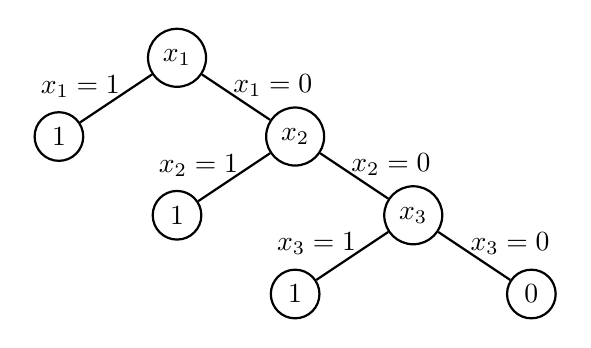
\begin{tikzpicture}
  [
    scale = 1, transform shape, thick,
    every node/.style = {draw, circle},
    grow = down,  % alignment of characters
    level 1/.style = {sibling distance=3cm},
    level 2/.style = {sibling distance=3cm}, 
    level distance = 1cm
  ]
  \node (Start) {$x_1$} 
   child { node (A1) {1}}
   child { node (A2) {$x_2$}
     child { node (B1) {1}}
     child { node (B2) {$x_3$}
        child { node (C1) {1}}
        child { node (C2) {0}}
     }
   };
  \begin{scope}[nodes = {draw = none}]
    \path (Start) -- (A1) node [near start, left]  {$x_1=1$};
    \path (Start) -- (A2) node [near start, right] {$x_1=0$};
    \path (A2) -- (B1) node [near start, left]  {$x_2=1$};
    \path (A2) -- (B2) node [near start, right] {$x_2=0$};
    \path (B2) -- (C1) node [near start, left]  {$x_3=1$};
    \path (B2) -- (C2) node [near start, right] {$x_3=0$};
  \end{scope}
\end{tikzpicture}
\end{center}
\item $f(x_1, x_2, x_3) = x_1 \land \neg x_2 \land \neg x_3$
\begin{center}
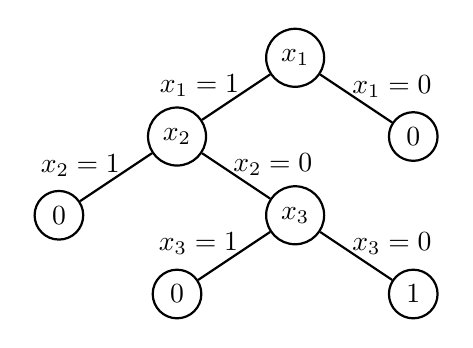
\begin{tikzpicture}
  [
    scale = 1, transform shape, thick,
    every node/.style = {draw, circle},
    grow = down,  % alignment of characters
    level 1/.style = {sibling distance=3cm},
    level 2/.style = {sibling distance=3cm}, 
    level distance = 1cm
  ]
  \node (Start) {$x_1$} 
   child { node (A1) {$x_2$}
     child { node (B1) {0}}
     child { node (B2) {$x_3$}
        child { node (C1) {0}}
        child { node (C2) {1}}
        }
   }
   child { node (A2) {0}};
  \begin{scope}[nodes = {draw = none}]
    \path (Start) -- (A1) node [near start, left]  {$x_1=1$};
    \path (Start) -- (A2) node [near start, right] {$x_1=0$};
    \path (A1) -- (B1) node [near start, left]  {$x_2=1$};
    \path (A1) -- (B2) node [near start, right] {$x_2=0$};
    \path (B2) -- (C1) node [near start, left]  {$x_3=1$};
    \path (B2) -- (C2) node [near start, right] {$x_3=0$};
  \end{scope}
\end{tikzpicture}
\end{center}
\item $f(x_1, x_2, x_3) = \neg x_1 \lor \neg x_2 \lor \neg x_3$
\begin{center}
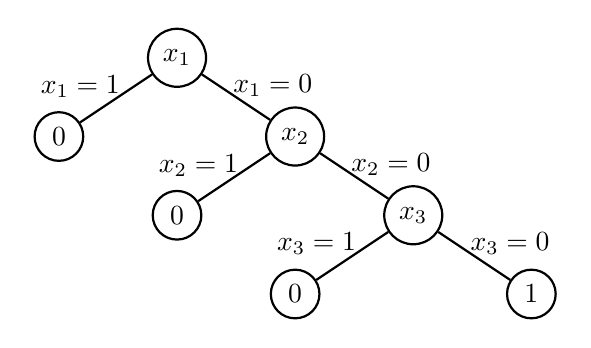
\begin{tikzpicture}
  [
    scale = 1, transform shape, thick,
    every node/.style = {draw, circle},
    grow = down,  % alignment of characters
    level 1/.style = {sibling distance=3cm},
    level 2/.style = {sibling distance=3cm}, 
    level distance = 1cm
  ]
  \node (Start) {$x_1$} 
   child { node (A1) {0}}
   child { node (A2) {$x_2$}
     child { node (B1) {0}}
     child { node (B2) {$x_3$}
        child { node (C1) {0}}
        child { node (C2) {1}}
     }
   };
  \begin{scope}[nodes = {draw = none}]
    \path (Start) -- (A1) node [near start, left]  {$x_1=1$};
    \path (Start) -- (A2) node [near start, right] {$x_1=0$};
    \path (A2) -- (B1) node [near start, left]  {$x_2=1$};
    \path (A2) -- (B2) node [near start, right] {$x_2=0$};
    \path (B2) -- (C1) node [near start, left]  {$x_3=1$};
    \path (B2) -- (C2) node [near start, right] {$x_3=0$};
  \end{scope}
\end{tikzpicture}
\end{center}
\item $f(x_1, x_2, x_3, x_4) = (x_1 \lor x_2) \land (x_3 \lor x_4)$
\begin{center}
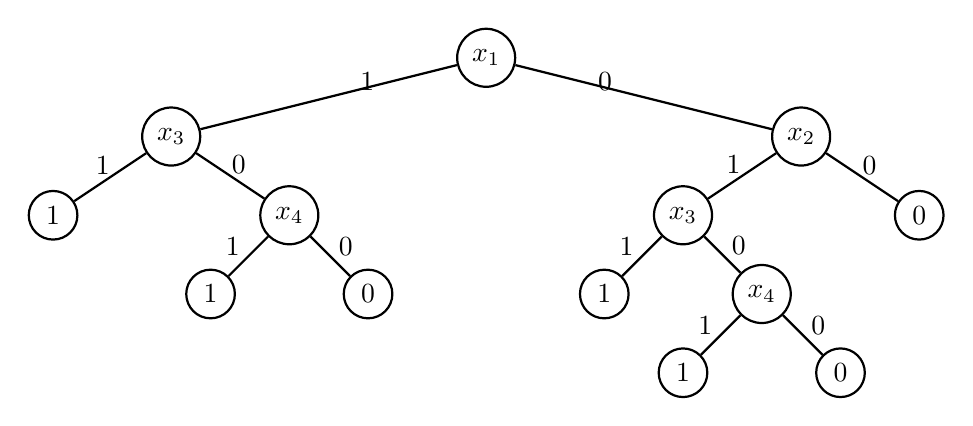
\begin{tikzpicture}
  [
    scale = 1, transform shape, thick,
    every node/.style = {draw, circle},
    grow = down,  % alignment of characters
    level 1/.style = {sibling distance=8cm},
    level 2/.style = {sibling distance=3cm}, 
    level 3/.style = {sibling distance=2cm}, 
    level 4/.style = {sibling distance=2cm}, 
    level distance = 1cm
  ]
  \node (Start) {$x_1$} 
   child { node (A) {$x_3$}
     child { node (AA) {1}}
     child { node (AB) {$x_4$}
       child { node (ABA) {1}}
       child { node (ABB) {0}}
     }
   }
   child { node (B) {$x_2$}
     child { node (BA) {$x_3$}
       child { node (BAA) {1}}
       child { node (BAB) {$x_4$}
         child { node (BABA) {1}}
         child { node (BABB) {0}}
       }
     }
     child { node (BB) {0}}
   };
  \begin{scope}[nodes = {draw = none}]
    \path (Start) -- (A) node [near start, left]  {1};
    \path (Start) -- (B) node [near start, right] {0};
    \path (A) -- (AA) node [near start, left] {1};
    \path (A) -- (AB) node [near start, right] {0};
    \path (AB) -- (ABA) node [near start, left] {1};
    \path (AB) -- (ABB) node [near start, right] {0};
    \path (B) -- (BA) node [near start, left] {1};
    \path (B) -- (BB) node [near start, right] {0};
    \path (BA) -- (BAA) node [near start, left] {1};
    \path (BA) -- (BAB) node [near start, right] {0};
    \path (BAB) -- (BABA) node [near start, left] {1};
    \path (BAB) -- (BABB) node [near start, right] {0};
  \end{scope}
\end{tikzpicture}
\end{center}
\item $f(x_1, x_2, x_3, x_4) = (x_1 \land x_2) \lor (x_3 \land x_4)$
\begin{center}
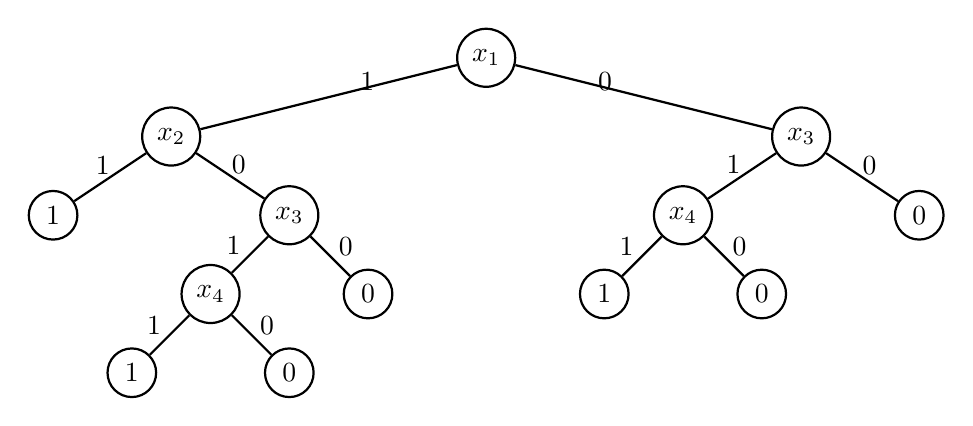
\begin{tikzpicture}
  [
    scale = 1, transform shape, thick,
    every node/.style = {draw, circle},
    grow = down,  % alignment of characters
    level 1/.style = {sibling distance=8cm},
    level 2/.style = {sibling distance=3cm}, 
    level 3/.style = {sibling distance=2cm}, 
    level 4/.style = {sibling distance=2cm}, 
    level distance = 1cm
  ]
  \node (Start) {$x_1$} 
   child { node (A) {$x_2$}
     child { node (AA) {1}}
     child { node (AB) {$x_3$}
       child { node (ABA) {$x_4$}
         child { node (ABAA) {1}}
         child { node (ABAB) {0}}
       }
       child { node (ABB) {0}}
     }
   }
   child { node (B) {$x_3$}
     child { node (BA) {$x_4$}
       child { node (BAA) {1}}
       child { node (BAB) {0}}
     }
     child { node (BB) {0}}
   };
  \begin{scope}[nodes = {draw = none}]
    \path (Start) -- (A) node [near start, left]  {1};
    \path (Start) -- (B) node [near start, right] {0};
    \path (A) -- (AA) node [near start, left] {1};
    \path (A) -- (AB) node [near start, right] {0};
    \path (AB) -- (ABA) node [near start, left] {1};
    \path (AB) -- (ABB) node [near start, right] {0};
    \path (ABA) -- (ABAA) node [near start, left] {1};
    \path (ABA) -- (ABAB) node [near start, right] {0};
    \path (B) -- (BA) node [near start, left] {1};
    \path (B) -- (BB) node [near start, right] {0};
    \path (BA) -- (BAA) node [near start, left] {1};
    \path (BA) -- (BAB) node [near start, right] {0};
  \end{scope}
\end{tikzpicture}
\end{center}
\end{enumerate}
\item~[10 points] Decision tree is \textbf{more expressive} than linear classifier. Decision tree can represent any boolean function but linear classifier cannot represent many non-trivial boolean functions such as parity.
\item~[30 points]
\begin{enumerate}
\item $f(x_1, x_2) = (x_1 \land \neg x_2) \lor (\neg x_1 \land x_2)$
$$z_1=x_1^2 \quad z_2=x_2^2 \quad z_3=x_1x_2$$
$$z_1+z_2-2z_3-1=0$$
\item $f(x_1, x_2) = (x_1 \land x_2) \lor (\neg x_1 \land \neg x_2)$
$$z_1=x_1^2 \quad z_2=x_2^2 \quad z_3=x_1x_2$$
$$-z_1-z_2+2z_3+1=0$$
\item $f(x_1, x_2, x_3)$
$$z_1=x_1 \quad z_2=x_2 \quad z_3=x_3 \quad z_4=[(x_1-x_2)^2-x_3]^2$$
$$z_4-1=0$$
\end{enumerate}
\item~[40 points]
\begin{enumerate}
\item~[10 points] $(\bx^\top \by)^2$
$$\phi(\bx) = [x_1^2,\ \sqrt{2}x_1x_2,\ x_2^2]$$
$$\phi(\by) = [y_1^2,\ \sqrt{2}y_1y_2,\ y_2^2]$$
\item~[10 points] $(\bx^\top \by)^3$
$$\phi(\bx) = [x_1^3,\ \sqrt{3}x_1^2x_2,\ \sqrt{3}x_1x_2^2,\ x_2^3]$$
$$\phi(\by) = [y_1^3,\ \sqrt{3}y_1^2y_2,\ \sqrt{3}y_1y_2^2,\ y_2^3]$$
\item~[20 points] $(\bf{x}^\top y)^k$ where $k$ is any positive integer.\\
According to \texttt{Yang Hui's triangle}, a.k.a. \texttt{Pascal's triangle}, the feature mappings are as follows,
\begin{align*}
&\phi(\bx)\\
=&\Big[\sqrt{t\choose0}x_1^t,\,\sqrt{t\choose1}x_1^{t-1}x_2,\,\sqrt{t\choose2}x_1^{t-2}x_2^2,\,\cdots,\,\sqrt{t\choose{t-1}}x_1x_2^{t-1},\,\sqrt{t\choose t}x_2^t\Big]
\end{align*}
\begin{align*}
&\phi(\by)\\
=&\Big[\sqrt{t\choose0}y_1^t,\,\sqrt{t\choose1}y_1^{t-1}y_2,\,\sqrt{t\choose2}y_1^{t-2}y_2^2,\,\cdots,\,\sqrt{t\choose{t-1}}y_1y_2^{t-1},\,\sqrt{t\choose t}y_2^t\Big]
\end{align*}
\end{enumerate}
\end{enumerate}

\section{Linear Regression}
\begin{enumerate}
\item~[10 points] Write down the LMS (least mean square) cost function $J(\bw, b)$.
\begin{align*}
J(\bw, b)=&\frac{1}{2}\sum_{x\in X}(y-(\bw^\top \bx+b))^2\\
=&\frac{1}{2}[(1-[1,-1,2]\bw-b)^2+(4-[1,1,3]\bw-b)^2+(-1-[-1,1,0]\bw-b)^2+\\&(-2-[1,2,-4]\bw-b)^2+(0-[3,-1,-1]\bw-b)^2]
\end{align*}
\item~[30 points] Calculate the gradient $\frac{\nabla J}{\nabla \bw}$ and $\frac{\nabla J}{\nabla b}$\\\\
The gradient can be calculated according to the formula,
$$\frac{\nabla J}{\nabla \bw}=\Big[\frac{\partial J}{\partial w_1},\frac{\partial J}{\partial w_2},\cdots,\frac{\partial J}{\partial w_d}\Big]$$
$$\frac{\partial J}{\partial w_j}=-\sum_{i=1}^m(y_i-\bw^\top\bx_i)x_{ij}$$
\begin{enumerate}
\item when $\bw = [0,0,0]^\top$ and $b = 0$;
$$\frac{\nabla J}{\nabla \bw}=[-4,2,-22],\quad\frac{\nabla J}{\nabla b}=-2$$
\item when $\bw = [-1,1,-1]^\top$ and $b = -1$;
$$\frac{\nabla J}{\nabla \bw}=[-22,16,-56],\quad\frac{\nabla J}{\nabla b}=-10$$
\item when $\bw = [1/2,-1/2,1/2]^\top$ and $b = 1$.
$$\frac{\nabla J}{\nabla \bw}=[7.5,-4,-5],\quad\frac{\nabla J}{\nabla b}=4.5$$
\end{enumerate}
\textbf{The code I used is in the appendix}.
\item~[20 points] What are the optimal $\bw$ and $b$ that minimize the cost function? 
$$\bw=[1,1,1]\quad b=-1$$
\textbf{The code I used is in the appendix}.
\item~[50 points]
\begin{enumerate}
\item Step1
$$\frac{\nabla J}{\nabla \bw}=[1,-1,2],\quad\frac{\nabla J}{\nabla b}=1$$
$$\bw=[0.1000,-0.1000,0.2000],\quad b=0.1000$$
\item Step2
$$\frac{\nabla J}{\nabla \bw}=[3.3000,3.3000,9.9000],\quad\frac{\nabla J}{\nabla b}=3.3000$$
$$\bw=[0.4300,0.2300,1.1900],\quad b=0.4300$$
\item Step3
$$\frac{\nabla J}{\nabla \bw}=[1.2300,-1.2300,0],\quad\frac{\nabla J}{\nabla b}=-1.2300$$
$$\bw=[0.5530,0.1070,1.1900],\quad b=0.3070$$
\item Step4
$$\frac{\nabla J}{\nabla \bw}=[1.6860,3.3720,-6.7440],\quad\frac{\nabla J}{\nabla b}=1.6860$$
$$\bw=[0.7216,0.4442,0.5156],\quad b=0.4756$$
\item Step5
$$\frac{\nabla J}{\nabla \bw}=[-5.0418,1.6806,1.6806],\quad\frac{\nabla J}{\nabla b}=-1.6806$$
$$\bw=[0.2174,0.6123,0.6837],\quad b=0.3075$$
\textbf{The code I used is in the appendix}.
\end{enumerate}
\end{enumerate}

\section{Mistake Driven Learning Algorithm}
\begin{enumerate}
\item~[10 points] Disjunction of $n$ boolean variables.\\\\
Taking negation into consideration, 
$$|C|=3^n \qquad M_A(C)=\log_2(3^n)=O(n)$$
$M_A(C)$ is polynomial to n. Thus Halving algorithm is a mistake bound algorithm for this concept class.
\item~[10 points] Disjunction of $k$ boolean variables out of the total $n$ input variables.\\\\
Taking negation into consideration, 
$$|C|={n\choose k}2^k\approx2^kn^k \qquad M_A(C)=\log_2(2^kn^k)=k+k\log_2n=O(k\log_2n)$$
$M_A(C)$ is logarithm of n, which is better than polynomial. Thus Halving algorithm is a mistake bound algorithm for this concept class.
\item~[10 points] $m$-of-$n$ rules. Note $m$ is a constant and smaller than $n$.\\\\
\textbf{It is ambiguous whether $m$ is a fixed number.}\\
If $m$ is any constant $m\in[n]$,
$$|C|=\sum_{i=1}^{n}i{n\choose k}=n\cdot2^{n-1}$$
$$M_A(C)=\log_2(n\cdot2^{n-1})=(n-1)\log_2n=O(n\log_2n)$$
If $m$ is a fixed constant $m\in[n]$,
$$|C|=m{n\choose m}\approx mn^m$$
$$M_A(C)=\log_2(mn^m)=\log_2m+m\log_2n=O(m\log_2n)$$
$M_A(C)$ is logarithm of n, which is better than polynomial. Thus Halving algorithm is a mistake bound algorithm for this concept class.
\item~[20 points] All boolean function of $n$ input boolean variables.
$$|C|=2^{2^n}$$
$$M_A(C)=\log_2(2^{2^n})=2^n=O(2^n)$$
$M_A(C)$ is exponential of n, which is worse than polynomial. Thus Halving algorithm is NOT a mistake bound algorithm for this concept class.
\end{enumerate}

\section{Perceptron}
\begin{enumerate}
\item  Let us review the Mistake Bound Theorem discussed in our lecture. 
\begin{enumerate}
\item~[10 points]\\\\
Given that,
$$\bu^\top\bw_t\ge t\gamma \qquad ||\bw||^2\le tR^2$$
We have,
$$t\gamma \le \bu^\top\bw_t \le ||\bu||\cdot||\bw_t|| \le ||\bu||\sqrt{t}R$$
Thus,
$$(\frac{R}{\gamma})^2\cdot||\bu||^2$$
\item~[10 points]
\begin{align*}
\gamma &= \min_{x_i\in X}\mathbf{dist}(x_i, h)\\
&= \min_{x_i\in X}\frac{\bu^\top\bx_iy_i}{||u||}\\
\gamma &\le \frac{y_i(\bu^\top\bx_i)}{||\bu||}
\end{align*}
\item~[20 points]\\\\
\textbf{The conclusion is the upper bound is still $(\cfrac{R}{\gamma})^2$}.
\begin{enumerate}
\item Proof 1/3 - After t mistakes, $\cfrac{\bu^\top\bw_t}{||\bu||} \ge t\gamma$\\
For t = 0,
$$\cfrac{\bu^\top\bw_t}{||\bu||} = t\gamma = 0$$
Assuming $t=t$ holds, for $t=t+1$,
\begin{align*}
\cfrac{\bu^\top\bw_t}{||\bu||} &= \frac{\bu^\top(\bw_t+\bx_iy_i)}{||\bu||}\\
&= \underbrace{\frac{\bu^\top\bw_t}{||\bu||}}_\text{$\ge t\gamma$} + \underbrace{\frac{\bu^\top\bx_iy_i}{||\bu||}}_\text{$\ge \gamma$}\\
& \ge (t+1)\gamma
\end{align*}
Thus, $\cfrac{\bu^\top\bw_t}{||\bu||} \ge t\gamma$ holds.
\item Proof 2/3 - After t mistakes, $||\bw_t||^2 \le tR^2$
$$\textbf{PROOF IS SAME AS BEFORE}$$
\item Proof 3/3 - $t \le (\cfrac{R}{\gamma})^2$
$$t\gamma \le \frac{\bu^\top\bw_t}{||\bu||} \le \frac{||\bu||\cdot||\bw_t||}{||\bu||}=||\bw_t|| \le \sqrt{t}R$$
$$t \le (\frac{R}{\gamma})^2$$
\end{enumerate}
\end{enumerate}
\item~[20 points]
A linear classifier for this disjunction is,
$$-x_1-x_2-\cdots-x_k+x_{k+1}+x_{k+2}+\cdots+x_{2k}+(k-\frac{1}{2})=0$$
Thus, the weight vector is,
$$\bw=(\underbrace{-1,-1,\cdots,-1}_\text{k},\underbrace{1,1,\cdots,1}_\text{k},\underbrace{0,0,\cdots,0}_\text{n-2k},k-\frac{1}{2})$$
$$||\bw||=\sqrt{2k+(k-\frac{1}{2})^2}=\sqrt{k^2+k+\frac{1}{4}}=\sqrt{(k+\frac{1}{2})^2}=k+\frac{1}{2}$$
$$\bw^\top\bx_iy_i\ge \frac{1}{2}$$
$$\gamma=min\frac{\bw^\top\bx_iy_i}{||\bw||}=\frac{\frac{1}{2}}{k+\frac{1}{2}}=\frac{1}{2k+1}$$
$$R=\sqrt{n+1}$$
The upper bound of the number of mistakes made by Perceptron in learning
this disjunction is,
$$(\frac{R}{\gamma})^2=\Big(\frac{\sqrt{n+1}}{\frac{1}{2k+1}}\Big)^2=(2k+1)^2(n+1)$$
This number is polynomial to input dimensionality n. So Perceptron is a mistake bound algorithm.
\end{enumerate}

\section{Programming Assignments}
\begin{enumerate}
\item Gradient Descent
\begin{enumerate}
\item~[90 points] Batch Gradient Descent\\
$$\bw=(0.90022, 0.78594, 0.85067, 1.29862, 0.12983, 1.57179, 0.99835, -0.01520)$$
$$\gamma=0.01$$
\begin{figure}[H]
\centering{
\includegraphics[width=.8\linewidth]{bgd.png}
}
\caption{Cost Function Value of Training Data at Each Step}
\label{fig:name}
\end{figure}
$$\mathcal{J}(\bw)=23.361305269196592$$
\item~[90 points] Stochastic Gradient Descent
$$\bw=(-0.07214, -0.25999, -0.23955, 0.51804, -0.03139, 0.24585, 0.01012, -0.03060)$$
$$\gamma=0.001$$
\begin{figure}[H]
\centering{
\includegraphics[width=.8\linewidth]{sgd.png}
}
\caption{Cost Function Value of Training Data at Each Step}
\label{fig:name}
\end{figure}
$$\mathcal{J}(\bw)=22.167107354823077$$
\item~[20 points] The optimal weight vector is,
$$\bw=(0.90056, 0.78629, 0.85104, 1.29889, 0.12989, 1.57225, 0.99869, -0.01520)$$
\begin{itemize}
\item Batch gradient descent will always converge to a solution that is close to the optimal solution while stochastic gradient descent won't.
\item Batch gradient descent requires less iteration to converge than stochastic gradient descent.
\item Stochastic gradient descent takes much less time than batch gradient descent at each step calculating the gradient and updating the weight vector.
\end{itemize}
\end{enumerate}
\item Perceptron
\begin{enumerate}
\item~[60 points] Standard perceptron
$$\bw=(-5.3207063, -3.563121, -4.4322626, -1.27922046, 5.7)$$
$$\text{Average prediction error: }0.02000$$
\item~[60 points] Voted perceptron\\\\
\textbf{Please find the learnt weight vectors in the appendix}.
$$\text{Average prediction error: }0.01400$$
\item~[60 points] Averaged perceptron
$$\bw=(-40225.7178191, -26477.132171, -27533.9904514, -7870.9174287, 34571.2)$$
$$\text{Average prediction error: }0.01400$$
\textbf{Observation: }Comparing to Voted Perceptron, Averaged Perceptron has the same prediction performance, but it does not have to store a large set of weight vectors, which dramatically reduces space consumption.
\item~[20 points]
\begin{itemize}
\item Generally speaking, Voted Perceptron and Average Perceptron have better prediction performance than Standard Perceptron.
\item Voted Perceptron and Average Perceptron have almost the same prediction performance, however, Averaged Perceptron takes much less space.
\end{itemize}
\end{enumerate}
\end{enumerate}

\newpage
\section{Appendix}
\subsection{Learnt Weight Vectors}
\begin{longtable}{c|c}
Weight Vector & Count\\
\hline
(0.00000,0.00000,0.00000,0.00000,0.00000) & 1 \\
(-0.58818,0.76584,0.05558,-0.29155,0.10000) & 3 \\
(-0.87209,0.10284,1.10407,-0.33366,0.20000) & 7 \\
(-0.86959,0.44282,0.66080,-0.76021,0.30000) & 2 \\
(-0.89462,-0.48980,1.02953,-0.13478,0.20000) & 4 \\
(-1.35901,-0.15251,0.76977,-0.19004,0.10000) & 3 \\
(-1.34733,0.22099,0.32598,-0.62745,0.20000) & 3 \\
(-1.21121,-0.84841,0.15576,-0.33719,0.10000) & 1 \\
(-1.26202,-0.56161,-0.02532,-0.56331,0.20000) & 4 \\
(-1.24888,-0.38386,-0.85848,-0.59852,0.10000) & 33 \\
(-1.42964,-1.26517,0.01238,-0.62021,0.20000) & 3 \\
(-1.38458,-1.12839,-0.69620,-0.57990,0.10000) & 13 \\
(-1.23562,-0.78551,-1.09929,-0.72249,0.20000) & 18 \\
(-1.56254,-2.05957,0.45644,-0.73668,0.30000) & 8 \\
(-1.81757,-1.56439,-0.18085,-0.69508,0.20000) & 10 \\
(-1.91054,-1.18468,-0.64514,-0.66551,0.10000) & 13 \\
(-1.69111,-0.72965,-1.14274,-0.93805,0.20000) & 13 \\
(-2.04792,-1.55095,-0.13444,-0.84128,0.30000) & 4 \\
(-1.92513,-1.14786,-0.59879,-1.23253,0.40000) & 8 \\
(-1.82319,-1.03757,-0.82879,-1.17314,0.50000) & 11 \\
(-1.87514,-0.71124,-1.13774,-1.07465,0.40000) & 2 \\
(-2.21096,-1.43528,0.00645,-1.13176,0.50000) & 9 \\
(-2.14047,-1.41811,-0.17214,-1.09564,0.60000) & 1 \\
(-2.10613,-1.40569,-0.20087,-1.08099,0.70000) & 13 \\
(-2.24032,-0.96348,-1.00987,-0.90750,0.60000) & 1 \\
(-2.27324,-0.51796,-1.46705,-0.80862,0.50000) & 5 \\
(-2.39892,-0.66529,-1.17987,-0.76397,0.60000) & 5 \\
(-2.77395,-2.01115,0.57945,-1.04168,0.70000) & 11 \\
(-2.90062,-1.72932,0.33685,-1.23030,0.80000) & 2 \\
(-3.06094,-1.25069,-0.51508,-1.01827,0.70000) & 3 \\
(-3.00914,-1.22483,-0.59917,-0.92215,0.80000) & 17 \\
(-2.95833,-1.17703,-0.79721,-0.86443,0.90000) & 11 \\
(-2.90210,-1.07688,-1.02447,-0.86504,1.00000) & 4 \\
(-2.89907,-1.18200,-0.88423,-0.78767,1.10000) & 44 \\
(-2.95102,-0.85567,-1.19318,-0.68918,1.00000) & 31 \\
(-2.70629,-2.11814,-1.26675,0.07694,0.90000) & 13 \\
(-2.79926,-1.73843,-1.73104,0.10651,0.80000) & 6 \\
(-2.66408,-1.63248,-1.96541,0.14651,0.90000) & 29 \\
(-2.46231,-1.45266,-2.26122,0.16750,1.00000) & 6 \\
(-2.60118,-1.94039,-1.61348,0.20168,1.10000) & 21 \\
(-2.45041,-1.74443,-1.91932,0.18943,1.20000) & 27 \\
(-2.34404,-1.37486,-2.33526,-0.00436,1.30000) & 2 \\
(-2.70320,-1.99771,-1.31137,-0.11979,1.40000) & 45 \\
(-2.54510,-1.91080,-1.54275,-0.03737,1.50000) & 13 \\
(-2.37711,-1.49012,-1.99673,-0.27668,1.60000) & 39 \\
(-2.13794,-1.03447,-2.49561,-0.56655,1.70000) & 2 \\
(-2.24538,-1.66560,-1.96011,-0.48608,1.80000) & 8 \\
(-2.60523,-3.03153,-0.19959,-0.73535,1.90000) & 1 \\
(-2.70064,-2.83329,-0.43122,-0.85492,2.00000) & 2 \\
(-2.79005,-2.51338,-0.61341,-1.14944,2.10000) & 7 \\
(-2.78343,-2.26424,-0.90742,-1.21160,2.20000) & 13 \\
(-3.02829,-1.63249,-1.70374,-1.23220,2.10000) & 56 \\
(-2.76350,-2.64623,-1.57064,-0.68513,2.00000) & 2 \\
(-2.74740,-1.99999,-2.40637,-0.53297,1.90000) & 11 \\
(-3.21505,-2.56635,-1.30947,-0.56642,2.00000) & 31 \\
(-3.15500,-2.37308,-1.63835,-0.59883,2.10000) & 52 \\
(-3.03420,-1.96564,-2.11470,-0.86012,2.20000) & 143 \\
(-2.83110,-1.78044,-2.41591,-0.85982,2.30000) & 26 \\
(-2.88305,-1.45411,-2.72486,-0.76133,2.20000) & 2 \\
(-2.61826,-2.46785,-2.59176,-0.21426,2.10000) & 9 \\
(-3.25190,-1.53937,-2.59033,-0.89270,2.20000) & 19 \\
(-3.24887,-1.64449,-2.45009,-0.81533,2.30000) & 32 \\
(-3.06303,-2.43309,-2.28366,-0.63149,2.20000) & 65 \\
(-2.88972,-2.03765,-2.75778,-0.88166,2.30000) & 28 \\
(-3.19838,-2.70127,-1.70373,-0.97085,2.40000) & 6 \\
(-3.04028,-2.61436,-1.93511,-0.88843,2.50000) & 15 \\
(-2.83851,-2.43454,-2.23092,-0.86744,2.60000) & 64 \\
(-2.87144,-1.98902,-2.68810,-0.76856,2.50000) & 1 \\
(-3.02466,-2.49868,-2.02031,-0.75107,2.60000) & 132 \\
(-3.07661,-2.17235,-2.32926,-0.65258,2.50000) & 107 \\
(-3.10953,-1.72683,-2.78644,-0.55370,2.40000) & 4 \\
(-2.92369,-2.51543,-2.62001,-0.36986,2.30000) & 23 \\
(-2.72059,-2.33023,-2.92122,-0.36956,2.40000) & 41 \\
(-3.12232,-3.16146,-1.67575,-0.51331,2.50000) & 10 \\
(-3.77316,-2.28450,-1.65256,-0.90701,2.60000) & 15 \\
(-3.60517,-1.86382,-2.10654,-1.14632,2.70000) & 41 \\
(-3.44613,-1.64261,-2.41837,-1.15804,2.80000) & 6 \\
(-3.77305,-2.91667,-0.86264,-1.17222,2.90000) & 3 \\
(-3.71300,-2.81672,-1.08390,-1.16248,3.00000) & 2 \\
(-3.49357,-2.36169,-1.58150,-1.43502,3.10000) & 5 \\
(-3.41488,-3.31832,-1.20283,-0.68468,3.00000) & 50 \\
(-3.66991,-2.82314,-1.84012,-0.64309,2.90000) & 17 \\
(-3.72186,-2.49681,-2.14907,-0.54460,2.80000) & 17 \\
(-3.65739,-2.03619,-2.98377,-0.27361,2.70000) & 26 \\
(-3.85148,-2.90467,-2.06827,-0.17956,2.80000) & 33 \\
(-3.78330,-2.41963,-2.58960,-0.78999,2.90000) & 90 \\
(-3.83524,-2.09330,-2.89855,-0.69150,2.80000) & 44 \\
(-4.14947,-3.39695,-1.33082,-0.75766,2.90000) & 13 \\
(-4.01764,-3.20678,-1.66193,-0.75115,3.00000) & 12 \\
(-3.89684,-2.79934,-2.13828,-1.01244,3.10000) & 69 \\
(-3.74788,-2.45646,-2.54137,-1.15503,3.20000) & 33 \\
(-3.73178,-1.81022,-3.37710,-1.00287,3.10000) & 10 \\
(-3.98843,-2.49846,-2.62294,-0.93210,3.20000) & 9 \\
(-4.04038,-2.17213,-2.93189,-0.83361,3.10000) & 41 \\
(-4.11025,-2.50984,-2.51978,-0.68318,3.20000) & 25 \\
(-4.14317,-2.06432,-2.97696,-0.58430,3.10000) & 5 \\
(-3.94007,-1.87912,-3.27817,-0.58400,3.20000) & 4 \\
(-4.01736,-2.62385,-2.62897,-0.54788,3.30000) & 46 \\
(-4.06931,-2.29752,-2.93792,-0.44939,3.20000) & 193 \\
(-4.44434,-3.64338,-1.17860,-0.72710,3.30000) & 9 \\
(-4.47141,-3.31664,-1.53422,-1.03598,3.40000) & 2 \\
(-4.37470,-2.93238,-2.02736,-1.44921,3.50000) & 35 \\
(-4.42665,-2.60605,-2.33631,-1.35072,3.40000) & 35 \\
(-4.25334,-2.21061,-2.81043,-1.60089,3.50000) & 50 \\
(-3.98855,-3.22435,-2.67733,-1.05382,3.40000) & 30 \\
(-3.78678,-3.04453,-2.97314,-1.03283,3.50000) & 133 \\
(-3.56735,-2.58950,-3.47074,-1.30537,3.60000) & 2 \\
(-4.04066,-3.20739,-2.33194,-1.41278,3.70000) & 4 \\
(-4.13363,-2.82768,-2.79623,-1.38321,3.60000) & 133 \\
(-4.05494,-3.78431,-2.41756,-0.63287,3.50000) & 38 \\
(-3.98676,-3.29927,-2.93889,-1.24330,3.60000) & 178 \\
(-3.97065,-2.65303,-3.77462,-1.09114,3.50000) & 10 \\
(-4.40941,-3.42570,-2.57807,-1.23657,3.60000) & 6 \\
(-4.46136,-3.09937,-2.88702,-1.13808,3.50000) & 47 \\
(-4.30232,-2.87816,-3.19885,-1.14980,3.60000) & 33 \\
(-4.35427,-2.55183,-3.50780,-1.05131,3.50000) & 10 \\
(-4.55493,-3.22373,-2.60618,-1.04132,3.60000) & 50 \\
(-4.49046,-2.76311,-3.44088,-0.77033,3.50000) & 155 \\
(-4.54241,-2.43678,-3.74983,-0.67183,3.40000) & 48 \\
(-4.68209,-3.40376,-2.80331,-0.70671,3.50000) & 37 \\
(-4.50334,-2.92576,-3.31693,-1.03033,3.60000) & 25 \\
(-4.30157,-2.74594,-3.61274,-1.00934,3.70000) & 29 \\
(-4.58548,-3.40894,-2.56425,-1.05145,3.80000) & 4 \\
(-4.67845,-3.02923,-3.02854,-1.02188,3.70000) & 2 \\
(-4.73040,-2.70290,-3.33749,-0.92339,3.60000) & 203 \\
(-4.52863,-2.52308,-3.63330,-0.90240,3.70000) & 45 \\
(-4.96636,-3.07475,-2.53940,-0.94322,3.80000) & 53 \\
(-4.95025,-2.42851,-3.37513,-0.79106,3.70000) & 12 \\
(-4.71108,-1.97286,-3.87401,-1.08093,3.80000) & 11 \\
(-4.52524,-2.76146,-3.70758,-0.89709,3.70000) & 10 \\
(-4.85216,-4.03552,-2.15185,-0.91127,3.80000) & 45 \\
(-4.70139,-3.83956,-2.45769,-0.92351,3.90000) & 24 \\
(-4.55243,-3.49668,-2.86078,-1.06610,4.00000) & 13 \\
(-4.37912,-3.10124,-3.33490,-1.31627,4.10000) & 130 \\
(-4.43107,-2.77491,-3.64385,-1.21778,4.00000) & 24 \\
(-4.80610,-4.12077,-1.88453,-1.49549,4.10000) & 2 \\
(-5.00086,-3.64339,-2.73723,-1.30881,4.00000) & 40 \\
(-4.79776,-3.45819,-3.03844,-1.30851,4.10000) & 74 \\
(-4.84971,-3.13186,-3.34739,-1.21002,4.00000) & 48 \\
(-4.90166,-2.80553,-3.65634,-1.11153,3.90000) & 19 \\
(-5.28369,-4.11104,-1.96051,-1.34205,4.00000) & 5 \\
(-5.18252,-4.02082,-2.19557,-1.29934,4.10000) & 1 \\
(-5.21544,-3.57530,-2.65275,-1.20046,4.00000) & 12 \\
(-5.08026,-3.46935,-2.88712,-1.16046,4.10000) & 26 \\
(-4.92216,-3.38245,-3.11850,-1.07805,4.20000) & 129 \\
(-4.95508,-2.93693,-3.57568,-0.97917,4.10000) & 116 \\
(-4.87639,-3.89356,-3.19701,-0.22883,4.00000) & 42 \\
(-4.65696,-3.43853,-3.69461,-0.50137,4.10000) & 73 \\
(-4.47821,-2.96053,-4.20823,-0.82499,4.20000) & 22 \\
(-4.82881,-4.21720,-2.69217,-0.90020,4.30000) & 45 \\
(-5.01097,-3.56972,-3.49731,-0.85835,4.20000) & 130 \\
(-4.86596,-3.20905,-3.90288,-1.01801,4.30000) & 117 \\
(-4.89888,-2.76353,-4.36006,-0.91913,4.20000) & 27 \\
(-5.36653,-3.32989,-3.26316,-0.95258,4.30000) & 11 \\
(-5.19322,-2.93445,-3.73728,-1.20275,4.40000) & 8 \\
(-4.99012,-2.74925,-4.03849,-1.20245,4.50000) & 39 \\
(-5.05613,-3.07185,-3.65791,-1.08409,4.60000) & 38 \\
(-5.10807,-2.74552,-3.96686,-0.98559,4.50000) & 3 \\
(-4.92223,-3.53412,-3.80043,-0.80175,4.40000) & 7 \\
(-4.68306,-3.07847,-4.29931,-1.09162,4.50000) & 32 \\
(-5.04222,-3.70132,-3.27542,-1.20705,4.60000) & 16 \\
(-5.02612,-3.05508,-4.11115,-1.05489,4.50000) & 95 \\
(-5.34035,-4.35873,-2.54342,-1.12106,4.60000) & 2 \\
(-5.39230,-4.03240,-2.85237,-1.02257,4.50000) & 56 \\
(-5.44425,-3.70607,-3.16132,-0.92408,4.40000) & 51 \\
(-5.49620,-3.37974,-3.47027,-0.82559,4.30000) & 26 \\
(-5.33716,-3.15853,-3.78210,-0.83731,4.40000) & 3 \\
(-5.09799,-2.70288,-4.28098,-1.12718,4.50000) & 1 \\
(-5.45715,-3.32573,-3.25709,-1.24261,4.60000) & 78 \\
(-5.29905,-3.23882,-3.48847,-1.16020,4.70000) & 138 \\
(-5.07962,-2.78379,-3.98607,-1.43274,4.80000) & 17 \\
(-5.14538,-3.06397,-3.61492,-1.33300,4.90000) & 50 \\
(-5.19733,-2.73764,-3.92387,-1.23451,4.80000) & 12 \\
(-5.39799,-3.40954,-3.02225,-1.22452,4.90000) & 88 \\
(-5.43092,-2.96402,-3.47943,-1.12564,4.80000) & 6 \\
(-5.48286,-2.63769,-3.78838,-1.02714,4.70000) & 125 \\
(-5.81868,-3.36173,-2.64419,-1.08426,4.80000) & 25 \\
(-5.91165,-2.98202,-3.10848,-1.05469,4.70000) & 11 \\
(-5.83296,-3.93865,-2.72981,-0.30435,4.60000) & 3 \\
(-5.80609,-3.43995,-3.24489,-0.94348,4.70000) & 71 \\
(-5.85804,-3.11362,-3.55384,-0.84499,4.60000) & 19 \\
(-5.69900,-2.89241,-3.86567,-0.85671,4.70000) & 85 \\
(-5.49590,-2.70721,-4.16688,-0.85641,4.80000) & 17 \\
(-5.85575,-4.07314,-2.40636,-1.10568,4.90000) & 7 \\
(-5.73495,-3.66570,-2.88271,-1.36697,5.00000) & 35 \\
(-5.56696,-3.24502,-3.33669,-1.60628,5.10000) & 16 \\
(-5.59988,-2.79950,-3.79387,-1.50740,5.00000) & 2 \\
(-5.52119,-3.75613,-3.41520,-0.75706,4.90000) & 27 \\
(-5.31942,-3.57631,-3.71101,-0.73607,5.00000) & 162 \\
(-5.08025,-3.12066,-4.20989,-1.02594,5.10000) & 127 \\
(-5.21912,-3.60839,-3.56215,-0.99176,5.20000) & 16 \\
(-5.27107,-3.28206,-3.87110,-0.89327,5.10000) & 31 \\
(-5.32302,-2.95573,-4.18005,-0.79478,5.00000) & 22 \\
(-5.52368,-3.62763,-3.27843,-0.78478,5.10000) & 45 \\
(-5.45921,-3.16701,-4.11313,-0.51379,5.00000) & 116 \\
(-5.78613,-4.44107,-2.55740,-0.52798,5.10000) & 2 \\
(-5.83808,-4.11474,-2.86635,-0.42949,5.00000) & 40 \\
(-5.89002,-3.78841,-3.17530,-0.33099,4.90000) & 96 \\
(-5.76922,-3.38097,-3.65165,-0.59228,5.00000) & 37 \\
(-5.80215,-2.93545,-4.10883,-0.49340,4.90000) & 40 \\
(-6.16200,-4.30138,-2.34831,-0.74267,5.00000) & 33 \\
(-6.13467,-3.81365,-2.84025,-1.32465,5.10000) & 3 \\
(-5.93290,-3.63383,-3.13606,-1.30366,5.20000) & 13 \\
(-5.78394,-3.29095,-3.53915,-1.44625,5.30000) & 41 \\
(-5.76783,-2.64471,-4.37488,-1.29409,5.20000) & 4 \\
(-6.14286,-3.99057,-2.61556,-1.57180,5.30000) & 29 \\
(-5.99785,-3.62990,-3.02113,-1.73146,5.40000) & 93 \\
(-5.79608,-3.45008,-3.31694,-1.71047,5.50000) & 4 \\
(-5.84802,-3.12375,-3.62589,-1.61198,5.40000) & 12 \\
(-5.66218,-3.91235,-3.45946,-1.42814,5.30000) & 12 \\
(-5.69511,-3.46683,-3.91664,-1.32926,5.20000) & 9 \\
(-5.61642,-4.42346,-3.53797,-0.57892,5.10000) & 41 \\
(-5.49363,-4.02037,-4.00232,-0.97017,5.20000) & 27 \\
(-5.52655,-3.57485,-4.45950,-0.87129,5.10000) & 115 \\
(-5.57850,-3.24852,-4.76845,-0.77280,5.00000) & 11 \\
(-5.98023,-4.07975,-3.52298,-0.91655,5.10000) & 41 \\
(-5.91576,-3.61913,-4.35768,-0.64556,5.00000) & 85 \\
(-5.96771,-3.29280,-4.66663,-0.54707,4.90000) & 3 \\
(-6.25162,-3.95580,-3.61814,-0.58918,5.00000) & 62 \\
(-6.09258,-3.73459,-3.92997,-0.60091,5.10000) & 57 \\
(-5.91383,-3.25659,-4.44359,-0.92453,5.20000) & 61 \\
(-6.24075,-4.53065,-2.88786,-0.93871,5.30000) & 31 \\
(-6.09574,-4.16998,-3.29343,-1.09837,5.40000) & 24 \\
(-5.92243,-3.77454,-3.76755,-1.34854,5.50000) & 43 \\
(-5.71933,-3.58934,-4.06876,-1.34824,5.60000) & 41 \\
(-5.77128,-3.26301,-4.37771,-1.24975,5.50000) & 13 \\
(-6.14089,-4.63080,-2.61976,-1.51156,5.60000) & 4 \\
(-5.97290,-4.21012,-3.07374,-1.75087,5.70000) & 8 \\
(-5.73373,-3.75447,-3.57262,-2.04074,5.80000) & 80 \\
(-5.65504,-4.71110,-3.19395,-1.29040,5.70000) & 34 \\
(-5.43561,-4.25607,-3.69155,-1.56294,5.80000) & 16 \\
(-5.52858,-3.87636,-4.15584,-1.53337,5.70000) & 239 \\
(-5.28941,-3.42071,-4.65472,-1.82324,5.80000) & 24 \\
(-5.69159,-4.25111,-3.39922,-1.97423,5.90000) & 14 \\
(-5.74354,-3.92478,-3.70817,-1.87574,5.80000) & 86 \\
(-5.58450,-3.70357,-4.02000,-1.88747,5.90000) & 3 \\
(-5.63645,-3.37724,-4.32895,-1.78898,5.80000) & 7 \\
(-5.66937,-2.93172,-4.78613,-1.69010,5.70000) & 5 \\
(-6.13275,-4.20681,-3.11447,-2.01178,5.80000) & 13 \\
(-6.18470,-3.88048,-3.42342,-1.91329,5.70000) & 34 \\
(-6.16859,-3.23424,-4.25915,-1.76113,5.60000) & 118 \\
(-6.08990,-4.19087,-3.88048,-1.01079,5.50000) & 23 \\
(-5.91659,-3.79543,-4.35460,-1.26096,5.60000) & 77 \\
(-5.94951,-3.34991,-4.81178,-1.16208,5.50000) & 15 \\
(-5.68472,-4.36365,-4.67868,-0.61501,5.40000) & 23 \\
(-5.73667,-4.03732,-4.98763,-0.51651,5.30000) & 179 \\
(-6.05972,-4.75867,-3.82330,-0.61113,5.40000) & 11 \\
\end{longtable}

\subsection{Code for Linear Regression Question}
\begin{lstlisting}[language=Matlab]
function result = gradient(w,x,y)
    result = zeros(1,length(w));
    for j=1:length(w)
        sum = 0;
        for i=1:length(x)
            disp(x(i,:))
            sum = sum + (y(i)-dot(w,x(i,:)))*x(i,j);
        end
        result(j) = -sum;
    end
end

function w = gradientDescent(x,y)
    w = [0 0 0 0];
    t = 0;
    while t < 1000
        w = w - 0.05 * gradient(w,x,y);
        t = t + 1;
    end
end

function w = stochasticGradientDescent(x,y)
    w = [0 0 0 0];
    t = 0;
    while t < 1
        for i=1:length(y)
            grad = zeros(1,length(w));
            for j=1:length(w)
                grad(j) = (y(i)-dot(w,x(i,:)))*x(i,j);
            end
            disp(grad)
            w = w + 0.1 * grad;
            disp(w)
        end
        t = t + 1;
    end
end
\end{lstlisting}
\end{document}